\section {Problem Introduction}
In the traditional Internet architecture, a single server handles multiple incoming client requests.  The bottleneck in such systems under high load can be lack of bandwidth to and from the server \cite{coopnet}, because bandwidth is split $N$ ways among the accessing clients (see Fig. \ref{fig:traditional_http}).  When an increasing number of users access a web page, that page therefore loads more and more slowly for users.  This circumstance occurs when server bandwidth is very low, a server experiences spikes in load, or multiple clients download very large files.  An example of this problem in real life is the ``slashdot" effect, in which a sudden flash crowd of clients suddenly request certain pages, overwhelming the unexpectant server (for example when linked to by the slashdot site).  These situations cause web servers to become overwhelmed and possibly crash.

This problem is most commonly combated by distributing the load among a set of servers that mirror the content of the original server (Fig. \ref{fig:server_only}).  A company establishes mirrors by locating a set of servers in many different places on the Internet, then automatically redirecting clients to these servers, thus distributing the load to provide better performance.  An example of this is the popular commercial CDN run by Akamai \cite{akamai}, which is employed to distribute large file downloads (for example Apple employs them to distribute their iTunes\texttrademark program).  This solution however requires a dedicated pool of servers to provide the extra bandwidth.  Not all sites can afford a CDN, and the mirrors require cooperation, configuration, and maintenance.

As a cheaper alternative, many web sites are beginning to use \emph{peer-to-peer content distribution}, or \emph{swarming}, with BitTorrent.  In BitTorrent, clients download only parts of a file from a central server, and get rest of it from their peers in the system.  While a client participates, it is both downloading the blocks it needs and uploading the blocks it has to other peers (see Fig. \ref{fig:normal_swarm}).  Peer-to-peer content distribution like this enables a web server to serve a large file to large numbers of users without overloading its server bandwidth \cite{zappala}. Swarming protocols have been shown to at times decrease total download time per peer as the number of peers increases \cite{slurpie}. 

\begin{figure}
\begin{center}
   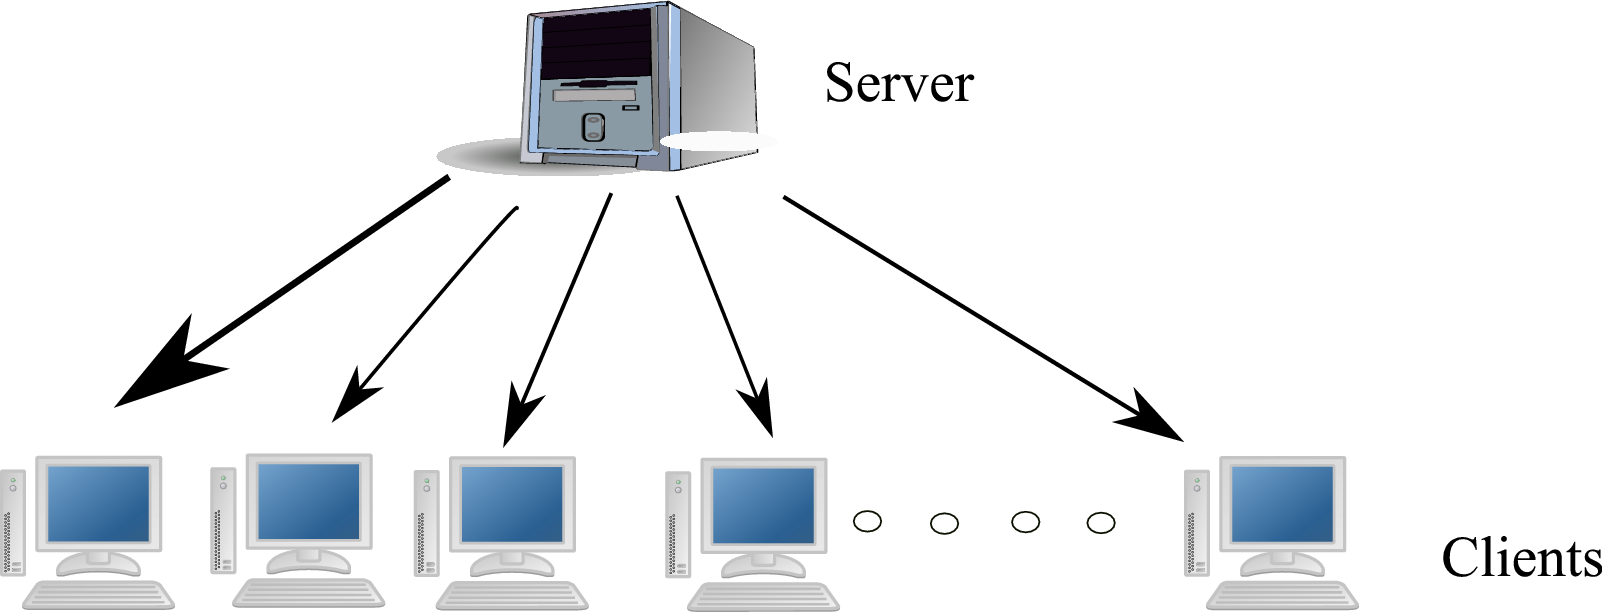
\includegraphics[width=11cm]{description_pics/traditional_http.png}
    \caption{Traditional HTTP download}
 \label{fig:traditional_http}
 \end{center}
\end{figure}
\begin{figure}
    \centering
  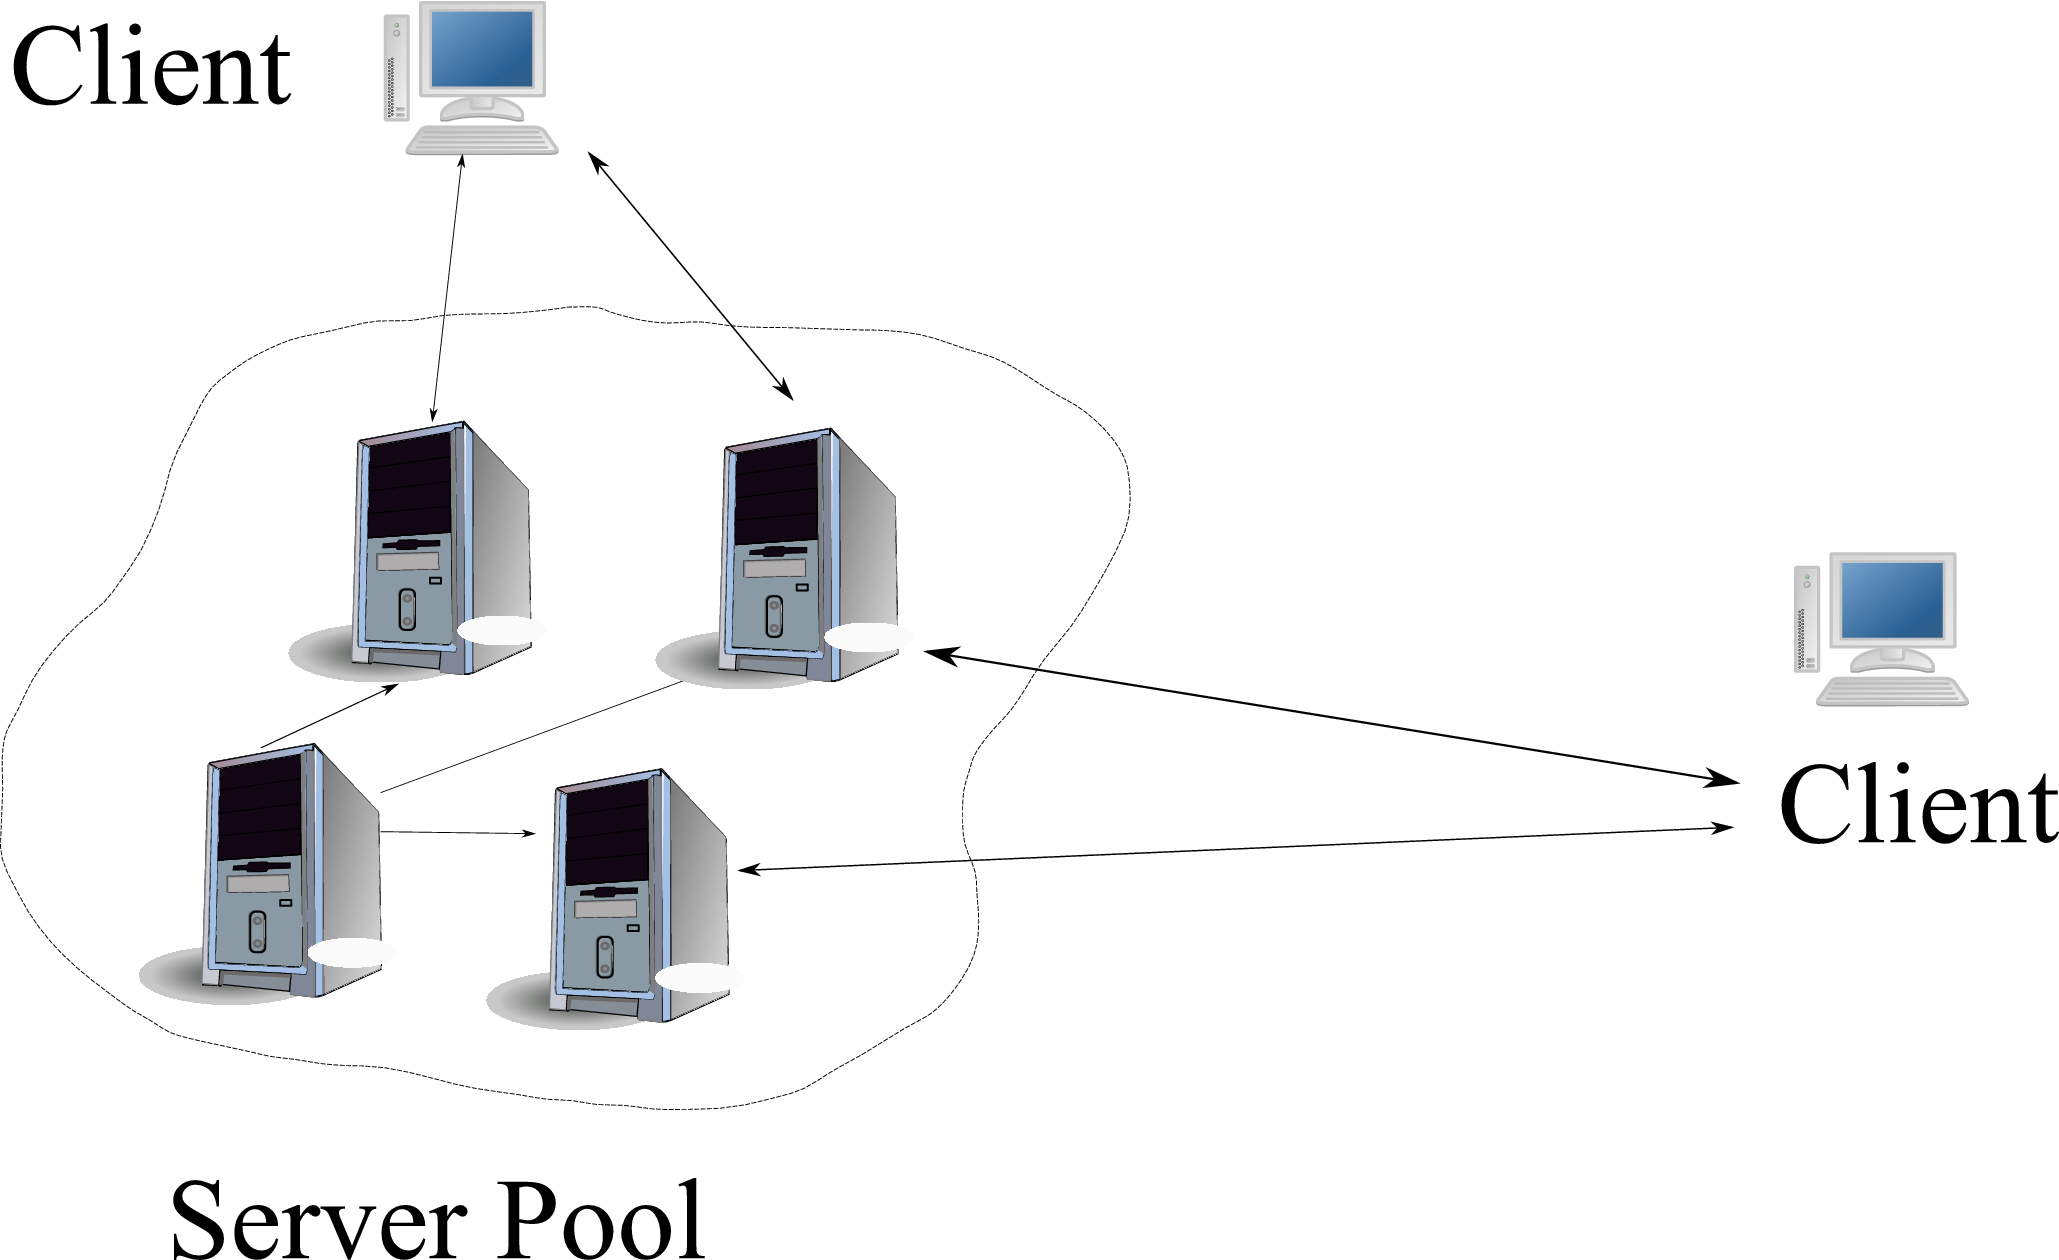
\includegraphics[width=8cm]{description_pics/server_side_only.png}
  \caption{Server CDN example}
  \label{fig:server_only}
\end{figure}   
\begin{figure}
 \centering
 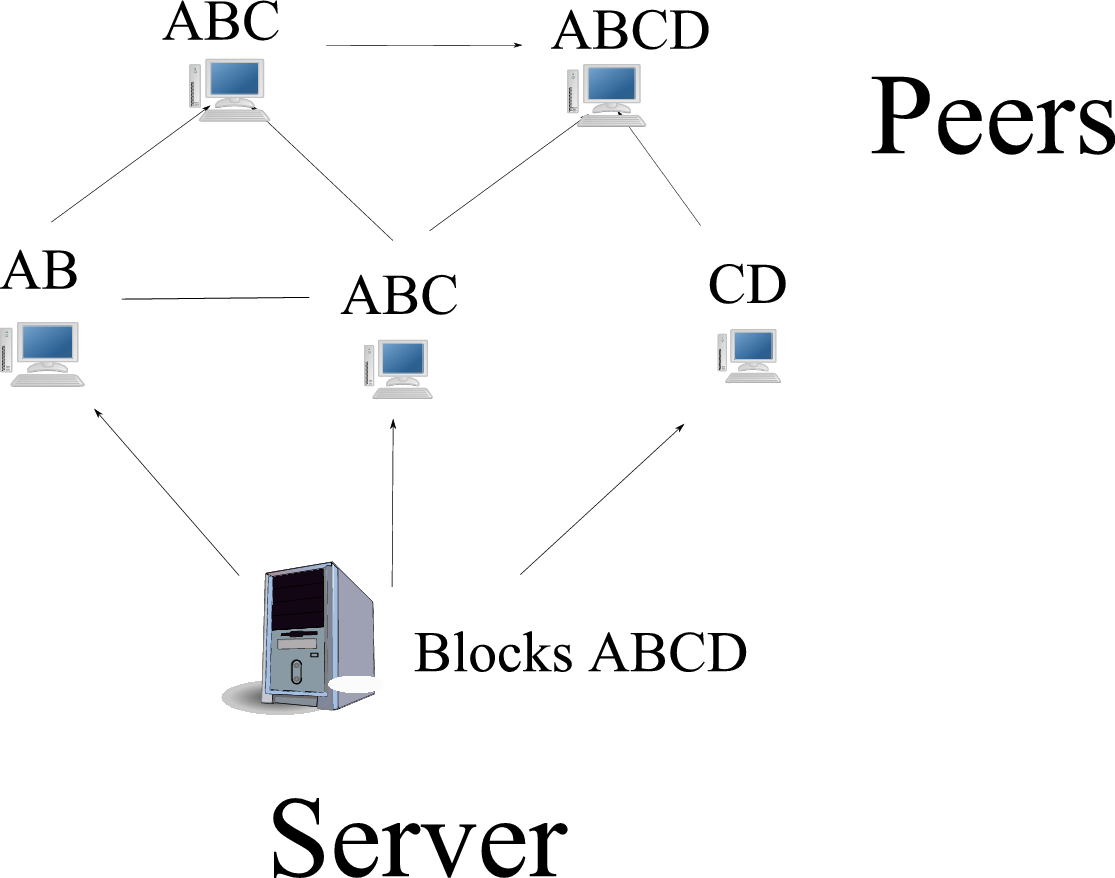
\includegraphics[width=4.5cm]{description_pics/normal_swarm.png}
 \caption{Swarming example.  Arrows represent block exchanges.}
 \label{fig:normal_swarm}
\end{figure}

BitTorrent currently requires setup for both servers and users, and isn't well-integrated into normal HTTP downloads.  BitTorrent peers must first locate a file with a ``.torrent'' extension from an out of band source such as a web server.  This file lists a target file's size, MD5 hashes of the blocks of the file, and the IP address of a tracker for that file.  This tracker is a machine which helps connect the peers to each another.  Peers contact the tracker to receive a list of peers who are currently downloading the file.  They then establish connections and begin sharing and receiving blocks with their neighbors.

%->final ?:BitTorrent, for the download of the last block of a file, uses a kind of 'many peers downloading the same blocks.  It requests the last block simultaneously from many peers, so that if one peer is transmitting it very slowly, they will be quickly passed by one of the faster seeds, and thus download it quickly.

BitTorrent is not commonly used for serving all the files of a web site.  It is used mostly for large files.  Every file shared has a .torrent file must be created, and a tracker established for that file\footnote{There have been some proposals of integrating BitTorrent with Apache \cite{webtorrent}, which show that even if a few clients contribute it helps with speedup, however this is mostly proposed as a server and client-side solution.  There are applets that will download BitTorrent files, and FireFox plugins to make downloading more seamless, but it still has a high barrier to entry for most users, and servers must understand the protocol.}.  This type of configuration is difficult for an entire web site, and unintuitive for small files.  Also, swarms are formed on a per file basis, which increases overhead.  BitTorrent also uses Tit-For-Tat incentives to share blocks of the same file, which can cause a longer boot-strapping time for new peers, and therefore is not as suited to small file downloads.  Recent improvements to BitTorrent include a ``trackerless'' option, which means peer lookup is shared amongst the peers themselves, but access to the original .torrent files is still centralized, requires an additional cost of setup for the web server, and peers must be BitTorrent capable.

Ideally, a web server would be able to automatically serve all its files using peer-to-peer file transfer if necessary, transitioning to peer-to-peer downloads based on the load it experiences.  This ``server-centric'' design would require that all web servers and clients know and use a peer-to-peer protocol, causing a barrier to entry.  Our protocol modifies web clients only, so that they transition to peer-to-peer download for files on any web server.  This client-side approach seens more feasible for widespread distribution.  The trade-offs of client-side and server-side protocols is discussed in more depth in the related works section.

\section {Thesis Statement}\label{section:thesis}
Our hypothesis is that a system of cooperating web clients can reduce load on an origin web server by automatically switching from client-server file transfer to peer-to-peer content delivery.  This system can provide fast download times for objects of many sizes, especially small files.  It should be equivalent in speed to BitTorrent for larger files, without requiring any manual configuration or participation from central web servers.

\section{Related Work}\label{section:related_work}
Much work has been done related to distributed file downloading.  Solutions fall into three basic categories: client-side protocols, client and server-side cooperative protocols, and server-side protocols.  Each category has certain trade-offs in terms of how it matches the ideal, above.

\subsection{Client-Side Only Protocols}
Protocols that use only client-side protocols help alleviate flash crowds.  Client-side interactions involve peers self-organizing to help speed downloads.  These solutions require no change in the server software, which allows them to be implemented in participating clients without requiring servers to be aware of the changes.  However, this requires that clients must self-organize without the help of the centralized server.  Our protocol is an example of such a system.

Shared web caches are another client-side answer to this problem.  They provide solutions for peers by allowing them to download files from some specified, well known cache of computers, such as Coral \cite{coral} or CoDeen \cite{codeen}, though such answers require a dedicated set of proxies.  Squirrel \cite{squirrel} is a shared web cache, however designed for use on a local LAN.  Squirrel clients join a DHT and cache any files that map to their location in the DHT.  The DHT is used to locate the peer owner who then serves as proxy for that file.  The advantage of this is it doesn't require dedicated infrastructure.  The disadvantage is it does not offer an algorithm for transparent transition to p2p download, always relying on the proxy for static content, and thus isn't suited for world-wide P2P sharing.  It also doesn't allow for partial file downloads.

Coral style caches have some disadvantages.  Advantages are that they reduce the load on the origin server, load balance among cache members, and are distributed over a wide area.  Disadvantages are that they are constrained to the number of participating proxies. They require an infrastructure of hosts who are willing to altruistically provide bandwidth, which is a rarity, and the only reason they are in existence is because of the Academic institutions who donate their bandwidth.  Requiring a dedicated infrastructure means that in extreme situations (load surpassing the bandwidth of the combined sum of computers), they still become overburdened (as an example, if Coral receives a request for a file too many times, it will begin redirecting peers back to the origin server, thus reverting to the original problem.  Coral is also limited in the size of files it can cache by PlanetLab policies.).  With our system this should not be a problem, as more peers means that more are also available for uploading.  Coral-style caches have their place, but are limited.  These systems also lack an algorithm for transition to peer-to-peer download.  They also add an extra hop in the network latency-wise, even if a request from the origin server would have been the fastest way to download the file.    
% we don't note that ``most web users aren't downloading, so could use that time to upload!'' -> future work

%The effect of  flash crowds can also be alleviated by searching among a random subset of Internet peers for desired files.  PROOFS \cite{proofs} (P2P Randomized Overlays to Obviate Flash-crowd Symptoms) uses flooded search to allow peers to locate 'popular' or 'flash crowded' files from other peers who have previously downloaded the same.  The creators conjecture that files that are the subjects of a flash crowd are likely to be locatable among random sets of peers, since they are popular, hence their use of a random flood search.  The benefit of this system is that nodes need not maintain a structured search system (such as a DHT). However, not having a DHT for lookup makes searches more random and slightly less accurate, with potentially higher overhead.  PROOFS also does not include parallel downloads nor offer a protocol for automatic transition to a peer-to-peer solution.

Overall, client-side solutions alleviate flash-crowds well, though they are limited in certain cases. There is also little automatic transition to peer-to-peer download.

\subsection{Server-side and Client-side Cooperative Protocols} 
%Many file distribution protocols include some cooperation and previous knowledge between the server and client.  In these protocols clients typically access blocks of a file from the server and also from peers.  Server-side and client-side cooperative protocols basically fall into two categories: those used for web redirection, and those used to download single objects.  For web redirection, servers typically redirect clients to former clients that have downloaded files previously \cite{pseudoserving, coopnet}.  This allows a server to 'meter' its upload speeds and redirect peers, when appropriate, thus providing a backup strategy for over-loaded servers.  An example of this is the pseudo-server system \cite{pseudoserving}.  This style of protocol typically requires changes to both the server and client software, however, and the server could still become overloaded in extreme cases.

Some protocols incorporate a type of redirection (i.e. the server redirects peers to recent downloaders), abd also include swarming capabilities \cite{overhaul, webtorrent, onion}.  Swarming provides the benefit of scalable downloads of large files.  OnionNetworks, for instance, proposes an extension to HTTP to allow HTTP response messages to include hashes of files and a list of peers from to which other peers may connect and download in a swarming fashion \cite{onion}.  Unfortunately their proposal has not seen wide-spread adoptance.  The use of swarming is a good principle, however, which we incorporate in our design.  Several protocols also initiate block-wise file distribution for arbitrary objects \cite{zappala, cohen, slurpie, mutualcast, fastreplica, avalanche, bullet_prime}.  BitTorrent, the most commonly used swarming protocol, was developed in 2001 by Bram Cohen \cite{cohen}.  Swarming protocols are highly effective in response to flash crowds, effectively serving loads orders of magnitude higher than an ordinary web server \cite{zappala}. As discussed above, it is still slightly centralized and requires extra setup for both client and server, thus hasn't seen wide-spread adoptance.

The Shark \cite{shark} filesystem allows clients to download blocks of files from nearby neighbors who have blocks already on their local machines. 
Shark is similar to our proposed system, except applied to files in a file system, not web objects.  It  requires a custom DHT for peer localization and proximity estimation, and a central server for hash values of files.  It also lacks HTTP integration and a switching mechanism.  Of other solutions, this one may be the closest to our design.

Some solutions seek to integrate HTTP clients with BitTorrent itself.  In these solutions a user is presented the option of downloading via HTTP or via BitTorrent (swarming), depending on which they think will give them the quicker download.  This provides a backup for overloaded servers.  To the users this requires a manual choice between normal to swarming download (and almost always normal download is faster, in the experience of the author).  The Osprey system \cite{osprey}, for example, is an ftp server that automatically generates .torrent files for all files in an ftp sub-directory, and integrates a BitTorrent tracker into the server software to handle the two types of requests.  Several other sites also offer .torrent files alongside normal (typically large) files, to allow users to manually use swarming in cases of high load.  These systems allow peers to manually switch to swarming if the server load becomes too high.  Dijjer \cite{dijjer} is a tool that automatically performs swarming downloads of any file.  If passed a url like http://dijjer.org/get/http://mysite.com/video.mov the request is intercepted by the Dijjer software, which performs a distributed download of the file.  One can also right-click on any arbitrary file and select 'download via Dijjer' for the same effect.  Dijjer contacts a quasi-DHT (similar to Freenet \cite{freenet}) for block hashes and downloads the blocks from random peers who cache these blocks.  Unfortunately, Dijjer lacks automation in the transition to download, and, as the Dijjer software is currently implemented, requires peers to cache material in which they were never interested, so is slightly intrusive.  Also their DHT seems slightly suspect for not being deterministic.  

Overall, client and server side cooperation protocols work well at alleviating flash crowds, and some provide automation for transition to p2p delivery.  However, they require both the server and client to understand the protocol, which hinders their adoptability.  The biggest drawback of these protocols is that they are not transparent to one side or the other.

\section {Proposed Solution}\label{section:solution}
Our proposed solution emphasizes a client-only system that automatically switches from client-server to a peer-to-peer content delivery without any manual per-file configuration for either clients or servers.  The goals for our system include:
\begin{enumerate}
\item It should be transparent to servers.  This allows the origin servers to remain unchanged, so end users can benefit from the system despite using servers who know nothing about it.
\item It should appear transparent to users by automatically transitioning to peer-to-peer content delivery when the server is slow.
\item It should not require a dedicated special-purpose infrastructure.  Using a general-purpose infrastructure, coupled with a dependence on the clients for transferring blocks, makes this system easier and cheaper to deploy.
\item It should be non-intrusive, in that peers should not be required to cache blocks of files in which they were never interested.  Peers will avoid caching files they never downloaded, and will not be responsible for content they don't anticipate.  Users would also only be using heir upload bandwidth for files in which they are interested, encouraging participation and adoption.
\item It should be fast for small files.
\end{enumerate}

%A fundamental design decision is also whether to download the contents of blocks from peers or from the DHT itself; peers could store the block contents, and have the DHT serve as a lookup of peers, or could store the block contents on the DHT itself.  The trade-off is that having the blocks on the DHT puts more stress on the DHT and relies on members of the DHT for contributing bandwidth, which is intrusive.  Imagine for instance caching portions of a file on your personal computer which you never downloaded for yourself, and which you are then sharing with others.  Members of the DHT would thus intrusively cache information for which they are not interested.  We therefore choose the case of having peers register themselves on a DHT as being willing to serve blocks they own, and have clients download directly from peers.  This seems more indicative of a realistic web experience.

